\documentclass[]{article}
\usepackage{amsfonts}
\usepackage{pgfplots}
\usetikzlibrary{math}
\usepackage{amsmath}
\usepackage{lmodern}
\usepackage[T1]{fontenc}
\usepackage{setspace}
%\usepackage{fullpage}
%\pgfplotsset{compat=1.15}

\renewcommand{\div}{\mathrm {div}}
\DeclareMathOperator{\curl}{curl}
\DeclareMathOperator{\ran}{ran}

\definecolor{newcolor}{RGB}{.8,.349,.1}
\definecolor{lightgray}{RGB}{200,200,200}
%%%%%emph colors
\definecolor{emph1}{RGB}{0,102,153}
\definecolor{emph2}{RGB}{200,90,20}
\definecolor{emph3}{RGB}{100,30,153}
\definecolor{emph4}{RGB}{0,100,0}
\definecolor{emph5}{RGB}{0,100,200}
\definecolor{emph6}{RGB}{100,0,0}

%for image output uncomment the following two lines and the pgf plot paragraph and compile with --shell-escape
\usepgfplotslibrary{external}
\tikzexternalize[prefix=images/]


\begin{document}


%%%%macros for drawing dofs
\newcommand{\trig}{%
  \draw[thick,gray](0,0)--++(4,0)--++(-4,4)--++(0,-4);
    \draw(0+2,0)--(0+4/3,0+4/3)--(0,0+2);
    \draw(0+2,0+2)--(0+4/3,0+4/3);
    }
\newcommand{\trigmethod}{%
  %\filldraw[fill=orange!30,thick,draw=gray](0,0)--++(4,0)--++(-4,4)--++(0,-4);
  \draw[thick](0,0)--++(4,0)--++(-4,4)--++(0,-4);
    %\filldraw[fill=orange!30](0+2,0)--(0+4/3,0+4/3)--(0,0+2);
    %\filldraw[fill=orange!30](0+2,0+2)--(0+4/3,0+4/3);
    \draw(0+2,0)--(0+4/3,0+4/3)--(0,0+2);
    \draw(0+2,0+2)--(0+4/3,0+4/3);
    \fill[fill=orange!30](0,0)--(0+2,0)--(0+4/3,0+4/3)--(0,0+2)--(0,0);
    }
\newcommand\dof[4][]{%
  \node[#1] at (2*#2-4/6*#2*#3,2*#3-4/6*#2*#3){};
  \node[] at (2*#2-4/6*#2*#3-0.1,2*#3-4/6*#2*#3-0.3){\small #4};
  %\node[#1] at (2*#3-4/6*#2*#3,4-2*#2+4/6*#2*#3-2*#3+4/6*#2*#3){};
  %\node[#1] at (4-2*#2+4/6*#2*#3-2*#3+4/6*#2*#3,2*#2-4/6*#2*#3){};
}
\newcommand\dofprimal[4][]{%
  \node[#1] at (2*#2-4/6*#2*#3,2*#3-4/6*#2*#3){};
  \node[] at (2*#2-4/6*#2*#3-0.1,2*#3-4/6*#2*#3-0.3){\small #4};
  \node[#1] at (2*#3-4/6*#2*#3,4-2*#2+4/6*#2*#3-2*#3+4/6*#2*#3){};
  \node[#1] at (4-2*#2+4/6*#2*#3-2*#3+4/6*#2*#3,2*#2-4/6*#2*#3){};
}
\newcommand\innerdofprimal[2]{
  \dofprimal[circle,thick,draw=blue]{#1}{#2}{}
}
\newcommand\innerdof[2]{
  \dof[circle,thick,draw=blue]{#1}{#2}{}
}
\newcommand\innervdof[2]{
  \dof[circle,thick,draw=teal]{#1}{#2}{}
}
\newcommand\graydof[2]{
  \dof[circle,thick,fill=gray]{#1}{#2}{}
}
\newcommand\graydofpimal[2]{
  \dofprimal[circle,thick,fill=gray]{#1}{#2}{}
}
\newcommand\facedof[2]{
  \dof[circle,fill=purple]{#1}{#2}{}
}
\newcommand\facedofprimal[2]{
  \dofprimal[circle,fill=purple]{#1}{#2}{}
}
\newcommand\facedoflabel[3]{
  \dof[circle,fill=purple]{#1}{#2}{#3}
}
\newcommand\edgedof[2]{
  \dof[circle,fill=blue]{#1}{#2}{}
}
\newcommand\edgedofprimal[2]{
  \dofprimal[circle,fill=blue]{#1}{#2}{}
}
\newcommand\edgedoflabel[3]{
  \dof[circle,fill=blue]{#1}{#2}{#3}
}
\newcommand\vertexdof[2]{
  \dof[circle,fill=teal]{#1}{#2}{}
}
\newcommand\vertexdofprimal[2]{
  \dofprimal[circle,fill=teal]{#1}{#2}{}
}
\newcommand\vertexdoflabel[3]{
  \dof[circle,fill=teal]{#1}{#2}{#3}
}
\newcommand\arrowdof[6][]{
  \begin{scope}[]
    \draw[#1,very thick,-latex] (2*#2-4/6*#2*#3,2*#3-4/6*#2*#3)--node {#6}                 (2*#4-4/6*#4*#5,2*#5-4/6*#4*#5);
  %\draw[#1,very thick,-latex] (2*#3-4/6*#2*#3,4-2*#2+4/6*#2*#3-2*#3+4/6*#2*#3)--(2*#5-4/6*#4*#5,4-2*#4+4/6*#4*#5-2*#5+4/6*#4*#5);
  %\draw[#1,very thick,-latex] (4-2*#2+4/6*#2*#3-2*#3+4/6*#2*#3,2*#2-4/6*#2*#3)--(4-2*#4+4/6*#4*#5-2*#5+4/6*#4*#5,2*#4-4/6*#4*#5);
  \end{scope}
}
\newcommand\arrowdofprimal[6][]{
  \begin{scope}[]
    \draw[#1,very thick,-latex] (2*#2-4/6*#2*#3,2*#3-4/6*#2*#3)--node {#6}                 (2*#4-4/6*#4*#5,2*#5-4/6*#4*#5);
  \draw[#1,very thick,-latex] (2*#3-4/6*#2*#3,4-2*#2+4/6*#2*#3-2*#3+4/6*#2*#3)--(2*#5-4/6*#4*#5,4-2*#4+4/6*#4*#5-2*#5+4/6*#4*#5);
  \draw[#1,very thick,-latex] (4-2*#2+4/6*#2*#3-2*#3+4/6*#2*#3,2*#2-4/6*#2*#3)--(4-2*#4+4/6*#4*#5-2*#5+4/6*#4*#5,2*#4-4/6*#4*#5);
  \end{scope}
}
\newcommand\facearrowdof[4]{
  \arrowdof[purple]{#1}{#2}{#3}{#4}{}
}
\newcommand\edgearrowdof[4]{
  \arrowdof[blue]{#1}{#2}{#3}{#4}{}
}
\newcommand\innerarrowdof[4]{
  \arrowdof[blue,dotted]{#1}{#2}{#3}{#4}{}
}

\newcommand\facearrowdofprimal[4]{
  \arrowdofprimal[purple]{#1}{#2}{#3}{#4}{}
}
\newcommand\edgearrowdofprimal[4]{
  \arrowdofprimal[blue]{#1}{#2}{#3}{#4}{}
}
\newcommand\innerarrowdofprimal[4]{
  \arrowdofprimal[blue,dotted]{#1}{#2}{#3}{#4}{}
}

\tikzsetnextfilename{ring_resonator_geo}
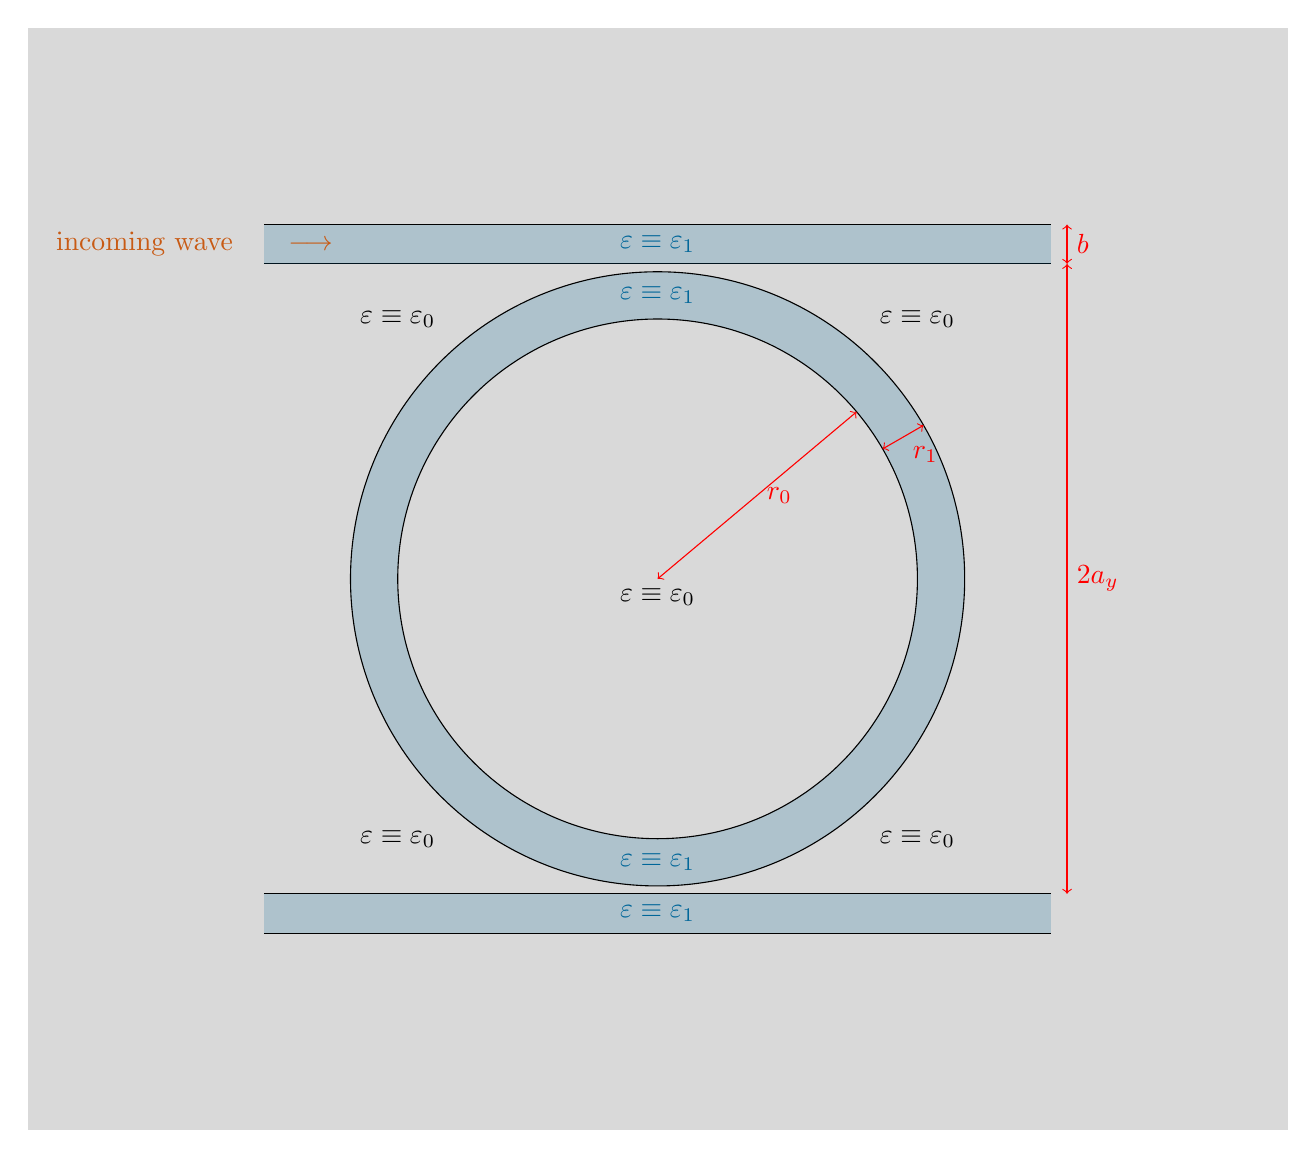
\begin{tikzpicture}
  \def\a{4};  
  \def\b{0.5};  
  \def\c{0.2};  
  \def\p{1};  
  \def\r{3.9};  
  \def\rr{3.3};  
  \def\bgx{-8};
  \def\bgxx{8};
  \def\bgy{-7}
  \def\bgyy{7}
  \fill[opacity=0.15] (\bgx,\bgy)rectangle(\bgxx,\bgyy);
  %\draw[] (-\a,-\a-\b-\c)--++(2*\a,0)--++(0,2*\a+2*\b+2*\c)--++(-2*\a,0)--++(0,-2*\a-2*\b-2*\c);
  %\draw[] (-\a-\p,\a)--++(2*\a+2*\p,0);
  \draw[] (-\a-\p,\a)--++(2*\a+2*\p,0);
  \draw[] (-\a-\p,\a+\b)--++(2*\a+2*\p,0);
  %\draw[] (-\a-\p,\a+\b+\c)--++(2*\a+2*\p,0);
  \draw[] (-\a-\p,-\a)--++(2*\a+2*\p,0);
  \draw[] (-\a-\p,-\a-\b)--++(2*\a+2*\p,0);
  %\draw[] (-\a-\p,-\a-\b-\c)--++(2*\a+2*\p,0);
  %\draw[] (-\a,-\a-\b-\c-\p)--++(-\p,\p)--++(0,2*\a+2*\b+2*\c)--++(\p,\p);
  %\draw[] (\a,-\a-\b-\c-\p)--++(\p,\p)--++(0,2*\a+2*\b+2*\c)--++(-\p,\p);
  %\fill[opacity=0.2] (\a,-\a-\b-\c-\p)--++(\p,\p)--++(0,2*\a+2*\b+2*\c)--++(-\p,\p);
  %\fill[opacity=0.2] (-\a,-\a-\b-\c-\p)--++(-\p,\p)--++(0,2*\a+2*\b+2*\c)--++(\p,\p);
  %\fill[opacity=0.2] (-\a,-\a-\b-\c-\p)--++(0,\p)--++(2*\a,0)--++(0,-\p);
  %\fill[opacity=0.2] (-\a,\a+\b+\c)--++(0,\p)--++(2*\a,0)--++(0,-\p);
  \fill[emph1,opacity=0.2] (-\a-\p,\a)--++(0,\b)--++(2*\a+2*\p,0)--++(0,-\b);
  \fill[emph1,opacity=0.2] (-\a-\p,-\a-\b)--++(0,\b)--++(2*\a+2*\p,0)--++(0,-\b);
  \fill[emph1,opacity=0.2,even odd rule] (0,0) circle (\r) (0,0) circle (\rr);
  \draw (0,0) circle (\r);
  \draw (0,0) circle (\rr);
  \node[left,emph2] at (-\a,\a+0.5*\b){incoming wave\qquad $\longrightarrow$};
  \node[emph1] at (0,\a+\b/2) {$\varepsilon\equiv\varepsilon_1$};
  \node[emph1] at (0,-\a-\b/2) {$\varepsilon\equiv\varepsilon_1$};
  \node[emph1] at (0,\r/2+\rr/2) {$\varepsilon\equiv\varepsilon_1$};
  \node[emph1] at (0,-\r/2-\rr/2) {$\varepsilon\equiv\varepsilon_1$};
  \node[below] at (0,0) {$\varepsilon\equiv\varepsilon_0$};
  \node[] at (\rr,\rr) {$\varepsilon\equiv\varepsilon_0$};
  \node[] at (-\rr,-\rr) {$\varepsilon\equiv\varepsilon_0$};
  \node[] at (-\rr,\rr) {$\varepsilon\equiv\varepsilon_0$};
  \node[] at (\rr,-\rr) {$\varepsilon\equiv\varepsilon_0$};
  %measurements
  %\draw[<->, red] (\a+\p+\c,\a+\b+\c+\p)--node[right]{$p$}++(0,-\p);
  %\draw[<->, red] (\a+\p+\c,\a+\b+\c)--node[right]{$c$}++(0,-\c);
  \draw[<->, red] (\a+\p+\c,\a+\b)--node[right]{$b$}++(0,-\b);
  \draw[<->, red] (\a+\p+\c,\a)--node[right]{$2a_y$}++(0,-\a-\a);
  %\draw[<->, red] (-\a,\a+\b+\c+\p+\c)--node[above]{$2a_x$}++(\a+\a,0);
  \draw[<->, red] (0,0)--node[right]{$r_0$}++(40:\rr);
  \draw[<->, red] (30:\rr)--node[below right]{$r_1$}(30:\r);
\end{tikzpicture}

\tikzsetnextfilename{ring_resonator_geo_pml}
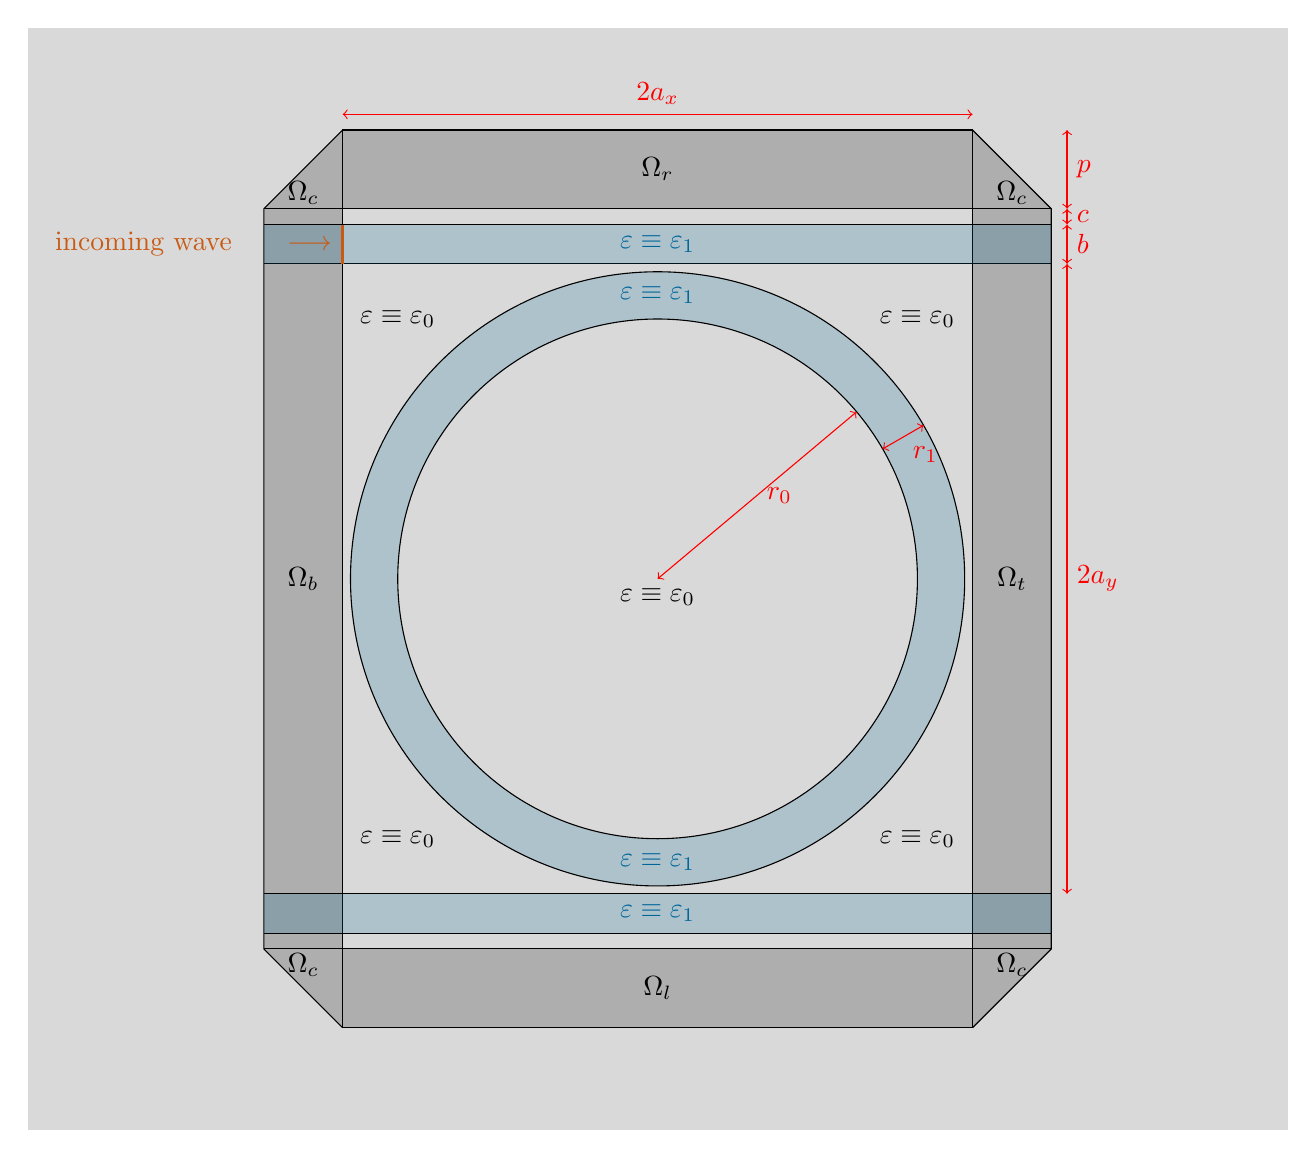
\begin{tikzpicture}
  \def\a{4};  
  \def\b{0.5};  
  \def\c{0.2};  
  \def\p{1};  
  \def\r{3.9};  
  \def\rr{3.3};  
  \def\bgx{-8};
  \def\bgxx{8};
  \def\bgy{-7}
  \def\bgyy{7}
  \fill[opacity=0.15] (\bgx,\bgy)rectangle(\bgxx,\bgyy);
  \draw[] (-\a,-\a-\b-\c-\p)--++(2*\a,0)--++(0,2*\a+2*\b+2*\c+2*\p)--++(-2*\a,0)--++(0,-2*\a-2*\b-2*\c-2*\p);
  \draw[] (-\a-\p,\a)--++(2*\a+2*\p,0);
  \draw[] (-\a-\p,\a)--++(2*\a+2*\p,0);
  \draw[] (-\a-\p,\a+\b)--++(2*\a+2*\p,0);
  \draw[] (-\a-\p,\a+\b+\c)--++(2*\a+2*\p,0);
  \draw[] (-\a-\p,-\a)--++(2*\a+2*\p,0);
  \draw[] (-\a-\p,-\a-\b)--++(2*\a+2*\p,0);
  \draw[] (-\a-\p,-\a-\b-\c)--++(2*\a+2*\p,0);
  \draw[] (-\a,-\a-\b-\c-\p)--++(-\p,\p)--++(0,2*\a+2*\b+2*\c)--++(\p,\p);
  \draw[] (\a,-\a-\b-\c-\p)--++(\p,\p)--++(0,2*\a+2*\b+2*\c)--++(-\p,\p);
  \fill[opacity=0.2] (\a,-\a-\b-\c-\p)--++(\p,\p)--++(0,2*\a+2*\b+2*\c)--++(-\p,\p);
  \fill[opacity=0.2] (-\a,-\a-\b-\c-\p)--++(-\p,\p)--++(0,2*\a+2*\b+2*\c)--++(\p,\p);
  \fill[opacity=0.2] (-\a,-\a-\b-\c-\p)--++(0,\p)--++(2*\a,0)--++(0,-\p);
  \fill[opacity=0.2] (-\a,\a+\b+\c)--++(0,\p)--++(2*\a,0)--++(0,-\p);
  \fill[emph1,opacity=0.2] (-\a-\p,\a)--++(0,\b)--++(2*\a+2*\p,0)--++(0,-\b);
  \fill[emph1,opacity=0.2] (-\a-\p,-\a-\b)--++(0,\b)--++(2*\a+2*\p,0)--++(0,-\b);
  \fill[emph1,opacity=0.2,even odd rule] (0,0) circle (\r) (0,0) circle (\rr);
  \draw (0,0) circle (\r);
  \draw (0,0) circle (\rr);
  \draw[very thick, emph2] (-\a,\a)--node[left]{incoming wave\qquad $\longrightarrow$}++(0,\b);
  \node at (0,\a+\b+\c+\p/2) {$\Omega_r$};
  \node at (0,-\a-\b-\c-\p/2) {$\Omega_l$};
  \node at (\a+\b+\c-\p/5,0) {$\Omega_t$};
  \node at (-\a-\b-\c+\p/5,0) {$\Omega_b$};
  \node at (-\a-\b-\c+\p/5,-\a-\b-\c-\p/5) {$\Omega_c$};
  \node at (+\a+\b+\c-\p/5,-\a-\b-\c-\p/5) {$\Omega_c$};
  \node at (-\a-\b-\c+\p/5,\a+\b+\c+\p/5) {$\Omega_c$};
  \node at (+\a+\b+\c-\p/5,\a+\b+\c+\p/5) {$\Omega_c$};
  \node[emph1] at (0,\a+\b/2) {$\varepsilon\equiv\varepsilon_1$};
  \node[emph1] at (0,-\a-\b/2) {$\varepsilon\equiv\varepsilon_1$};
  \node[emph1] at (0,\r/2+\rr/2) {$\varepsilon\equiv\varepsilon_1$};
  \node[emph1] at (0,-\r/2-\rr/2) {$\varepsilon\equiv\varepsilon_1$};
  \node[below] at (0,0) {$\varepsilon\equiv\varepsilon_0$};
  \node[] at (\rr,\rr) {$\varepsilon\equiv\varepsilon_0$};
  \node[] at (-\rr,-\rr) {$\varepsilon\equiv\varepsilon_0$};
  \node[] at (-\rr,\rr) {$\varepsilon\equiv\varepsilon_0$};
  \node[] at (\rr,-\rr) {$\varepsilon\equiv\varepsilon_0$};
  %measurements
  \draw[<->, red] (\a+\p+\c,\a+\b+\c+\p)--node[right]{$p$}++(0,-\p);
  \draw[<->, red] (\a+\p+\c,\a+\b+\c)--node[right]{$c$}++(0,-\c);
  \draw[<->, red] (\a+\p+\c,\a+\b)--node[right]{$b$}++(0,-\b);
  \draw[<->, red] (\a+\p+\c,\a)--node[right]{$2a_y$}++(0,-\a-\a);
  \draw[<->, red] (-\a,\a+\b+\c+\p+\c)--node[above]{$2a_x$}++(\a+\a,0);
  \draw[<->, red] (0,0)--node[right]{$r_0$}++(40:\rr);
  \draw[<->, red] (30:\rr)--node[below right]{$r_1$}(30:\r);
\end{tikzpicture}


\tikzsetnextfilename{stokes}
      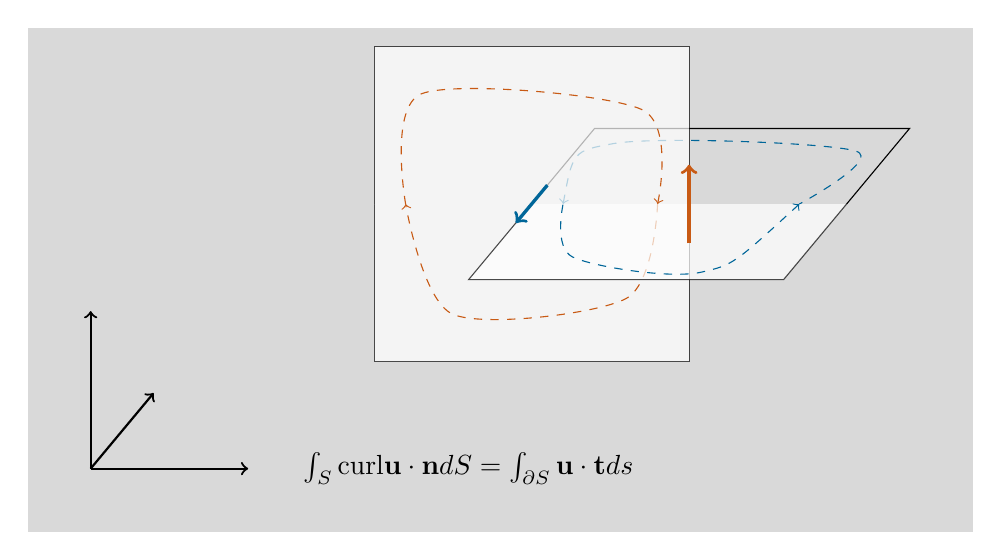
\begin{tikzpicture}[scale=0.8]
        \def\dxx{2.5};
        \def\dxy{0};
        \def\dyx{1};
        \def\dyy{1.2};
        \def\dzx{0};
        \def\dzy{2.5};
  \def\bgx{-7};
  \def\bgxx{8};
  \def\bgy{-4}
  \def\bgyy{4}
  \fill[opacity=0.15] (\bgx,\bgy)rectangle(\bgxx,\bgyy);
        \draw[fill=white,opacity=0.7] (-\dxx+\dyx,-\dxy+\dyy)
        --++(-\dzx,-\dzy)%--++(-\dzx,-\dzy)
        --++(2*\dxx,2*\dxy)
        --++(\dzx,\dzy);
        \draw[emph1,dashed,<-] plot [smooth]coordinates{(\dyx+0.2*\dxx,\dyy+0.1*\dxy)(2.3*\dyx,1.8*\dyy)(1.9*\dyx+1.7*\dxx,1.7*\dyy+1.8*\dxy)(\dyx+1.7*\dxx,\dyy+1.9*\dxy)};
        \draw (2*\dxx+\dyx,2*\dxy+\dyy)
        --++(\dyx,\dyy)
        --++(-\dxx,-\dxy)--++(-\dxx,-\dxy)
        --++(-\dyx,-\dyy);
        %\draw[fill=white,opacity=0.7] (\dxx+\dyx,\dxy+\dyy)
        %--++(\dzx,\dzy)%--++(\dzx,\dzy)
        %--++(\dyx,\dyy)--++(\dyx,\dyy)
        %--++(-\dzx,-\dzy)%--++(-\dzx,-\dzy)
        %--++(-\dyx,-\dyy)--cycle;
        \draw[fill=white,opacity=0.7] (-\dxx+\dyx,-\dxy+\dyy)
        --++(\dzx,\dzy)%--++(\dzx,\dzy)
        --++(\dxx,\dxy)--++(\dxx,\dxy)
        --++(-\dzx,-\dzy);%--++(-\dzx,-\dzy)
        \draw[emph2,dashed,->] plot [smooth]coordinates{(0.8*\dxx+\dyx,\dxy+\dyy)(0.6*\dxx+\dyx-\dzx,\dxy+\dyy-0.6*\dzy)(-0.5*\dxx+\dyx-0.6*\dzx,-\dxy+\dyy-0.7*\dzy)(-0.8*\dxx+\dyx,-0.8*\dxy+\dyy)};
        \draw[fill=white,opacity=0.7] (2*\dxx+\dyx,2*\dxy+\dyy)
        --++(-\dyx,-\dyy)
        --++(-\dxx,-\dxy)--++(-\dxx,-\dxy)
        --++(\dyx,\dyy);
        \draw[emph1,dashed,<-] plot [smooth]coordinates{(\dyx+1.7*\dxx,\dyy+1.9*\dxy)(0.2*\dyx+1.4*\dxx,0.1*\dyy+1.7*\dxy)(0.4*\dyx+0.5*\dxx,0.3*\dyy+0.1*\dxy)(\dyx+0.2*\dxx,\dyy+0.1*\dxy)};
        \draw[emph2,dashed,->] plot [smooth]coordinates{(-0.8*\dxx+\dyx,-0.8*\dxy+\dyy)(-0.7*\dxx+\dyx+0.6*\dzx,-\dxy+\dyy+0.7*\dzy)(0.7*\dxx+\dyx+\dzx,\dxy+\dyy+0.6*\dzy)(0.8*\dxx+\dyx,\dxy+\dyy)};
        \draw[emph2,->,very thick] (\dxx+\dyx-0.25*\dzx,\dxy+\dyy-0.25*\dzy)--++(0.5*\dzx,0.5*\dzy);
        \draw[emph1,->,very thick] (1.25*\dyx,1.25*\dyy)--++(-0.5*\dyx,-0.5*\dyy);
        %\draw[gray, dashed] (.5,-5)--(0.5,1)--(2.5,4)--(2.5,-2)--(.5,-5);
        \draw[thick,->](-6,-3)--++(\dxx,\dxy);
        \draw[thick,->](-6,-3)--++(\dyx,\dyy);
        \draw[thick,->](-6,-3)--++(\dzx,\dzy);
        \node at (-0,-3){$\int_S \mathrm{curl} \mathbf{u} \cdot \mathbf{n} dS = \int_{\partial S} \mathbf{u}\cdot \mathbf t ds$};
      \end{tikzpicture}

      







\tikzsetnextfilename{stokes_disc}
      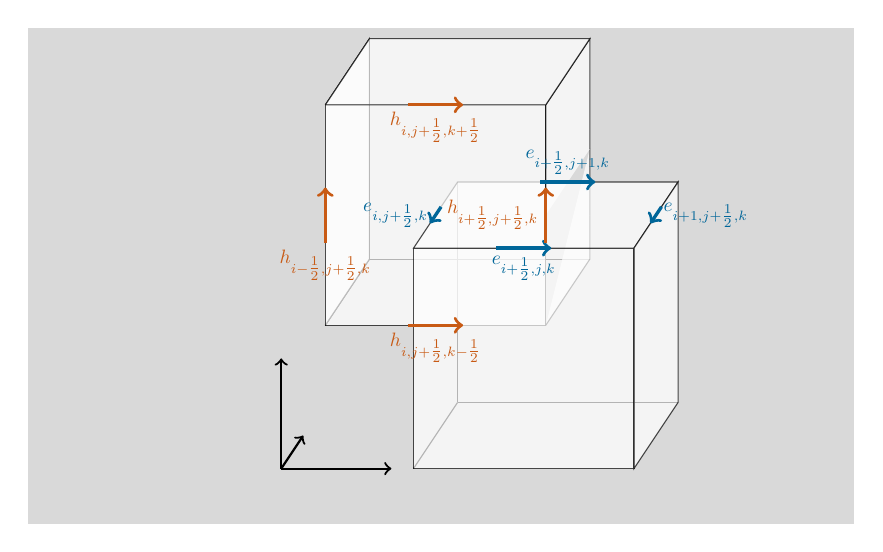
\begin{tikzpicture}[scale=0.7, every node/.style={transform shape}]
        \def\dxx{2};
        \def\dxy{0};
        \def\dyx{0.4};
        \def\dyy{0.6};
        \def\dzx{0};
        \def\dzy{2};
  \def\bgx{-7};
  \def\bgxx{8};
  \def\bgy{-5}
  \def\bgyy{4}
  \fill[opacity=0.15] (\bgx,\bgy)rectangle(\bgxx,\bgyy);
        %red invisible
        \draw (-\dxx+3*\dyx-\dzx,-\dxy+3*\dyy-\dzy)
        --++(2*\dzx,2*\dzy);
        \draw (-\dxx+3*\dyx-\dzx,-\dxy+3*\dyy-\dzy)
        --++(2*\dxx,2*\dxy);
        \draw (-\dxx+3*\dyx-\dzx,-\dxy+3*\dyy-\dzy)
        --++(-2*\dyx,-2*\dyy);
        %blue invisible
        \draw (2*\dyx,2*\dyy)
        --++(-2*\dzx,-2*\dzy);
        \draw (2*\dyx-2*\dzx,2*\dyy-2*\dzy)
        --++(-2*\dyx,-2*\dyy);
        \draw (2*\dyx-2*\dzx,2*\dyy-2*\dzy)
        --++(2*\dxx,2*\dxy);
        \draw[fill=white,opacity=0.7] (\dyx-\dzy,\dyy-\dzy)
        --++(2*\dyx,2*\dyy)%--++(-\dzx,-\dzy)
        --++(2*\dzx,2*\dzy)
        --++(-2*\dyx,-2*\dyy);
        \draw[fill=white,opacity=0.7] (2*\dxx+\dyx-\dzy,2*\dxy+\dyy-\dzy)
        --++(2*\dyx,2*\dyy)%--++(-\dzx,-\dzy)
        --++(\dzx,\dzy);
        \draw[fill=white,opacity=0.7] (-\dxx+\dyx,-\dxy+\dyy)
        --++(-\dzx,-\dzy)%--++(-\dzx,-\dzy)
        --++(2*\dxx,2*\dxy)
        --++(\dzx,\dzy);
        \draw[fill=white,opacity=0.7] (2*\dxx+\dyx,2*\dxy+\dyy)
        --++(\dyx,\dyy)
        --++(-\dxx,-\dxy)--++(-\dxx,-\dxy)
        --++(-\dyx,-\dyy);
        \draw[fill=white,opacity=0.7] (-\dxx+\dyx,-\dxy+\dyy)
        --++(\dzx,\dzy)%--++(\dzx,\dzy)
        --++(\dxx,\dxy)--++(\dxx,\dxy)
        --++(-\dzx,-\dzy);%--++(-\dzx,-\dzy)
        \draw[fill=white,opacity=0.7] (\dxx+\dyx,\dxy+\dyy)
        --++(\dzx,\dzy)%--++(-\dzx,-\dzy)
        --++(2*\dyx,2*\dyy)
        --++(-\dzx,-\dzy);
        \draw[fill=white,opacity=0.7] (2*\dxx+\dyx,2*\dxy+\dyy)
        --++(-\dyx,-\dyy)
        --++(-\dxx,-\dxy)--++(-\dxx,-\dxy)
        --++(\dyx,\dyy);
        %red top 
        \draw[fill=white,opacity=0.7] (-\dxx+\dzx+\dyx,-\dxy+\dzy+\dyy)
        --++(2*\dxx,2*\dxy)
        --++(2*\dyx,2*\dyy)
        --++(-2*\dxx,-2*\dxy)
        --++(-2*\dyx,-2*\dyy);

        %blue front, right
        \draw[fill=white,opacity=0.7] (0,0)
        --++(2*\dxx,2*\dxy)
        --++(-2*\dzx,-2*\dzy)
        --++(-2*\dxx,-2*\dxy)
        --++(2*\dzx,2*\dzy);
        \draw[fill=white,opacity=0.7] (2*\dxx,2*\dxy)
        --++(2*\dyx,2*\dyy)
        --++(-2*\dzx,-2*\dzy)
        --++(-2*\dyx,-2*\dyy)
        --++(2*\dzx,2*\dzy);



        \draw[emph1,->,very thick] (1.25*\dyx,1.25*\dyy)--node[left]{$e_{i,j+\tfrac{1}{2},k}$}++(-0.5*\dyx,-0.5*\dyy);
        \draw[emph1,->,very thick] (1.25*\dyx+2*\dxx,1.25*\dyy+2*\dxy)--node[right]{$e_{i+1,j+\tfrac{1}{2},k}$}++(-0.5*\dyx,-0.5*\dyy);
%        \draw[emph1,->,very thick] (1.25*\dyx-2*\dzx,1.25*\dyy-2*\dzy)--++(-0.5*\dyx,-0.5*\dyy);
%        \draw[emph1,->,very thick] (1.25*\dyx-2*\dzx+2*\dxx,1.25*\dyy-2*\dzy+2*\dxy)--++(-0.5*\dyx,-0.5*\dyy);
%
        \draw[emph1,->,very thick] (0.75*\dxx,0.75*\dxy)--node[below]{$e_{i+\tfrac{1}{2},j,k}$}++(0.5*\dxx,0.5*\dxy);
        \draw[emph1,->,very thick] (0.75*\dxx+2*\dyx,0.75*\dxy+2*\dyy)--node[above]{$e_{i+\tfrac{1}{2},j+1,k}$}++(0.5*\dxx,0.5*\dxy);
%        \draw[emph1,->,very thick] (0.75*\dxx+2*\dyx-2*\dzx,0.75*\dxy+2*\dyy-2*\dzy)--++(0.5*\dxx,0.5*\dxy);
%        \draw[emph1,->,very thick] (0.75*\dxx-2*\dzx,0.75*\dxy-2*\dzy)--++(0.5*\dxx,0.5*\dxy);
%
%        \draw[emph1,->,very thick] (-1.25*\dzx,-1.25*\dzy)--++(0.5*\dzx,0.5*\dzy);
%        \draw[emph1,->,very thick] (-1.25*\dzx+2*\dxx,2*\dxy-1.25*\dzy)--++(0.5*\dzx,0.5*\dzy);
%        \draw[emph1,->,very thick] (-1.25*\dzx+2*\dxx+2*\dyx,2*\dxy-1.25*\dzy+2*\dyy)--++(0.5*\dzx,0.5*\dzy);
%        \draw[emph1,->,very thick] (-1.25*\dzx+2*\dyx,-1.25*\dzy+2*\dyy)--++(0.5*\dzx,0.5*\dzy);
        \begin{scope}[shift={(-\dxx+\dyx+\dzx,-\dxy+\dyy+\dzy)}]
%          \draw[emph2,->,very thick] (1.25*\dyx,1.25*\dyy)--++(-0.5*\dyx,-0.5*\dyy);
%          \draw[emph2,->,very thick] (1.25*\dyx+2*\dxx,1.25*\dyy+2*\dxy)--++(-0.5*\dyx,-0.5*\dyy);
%          \draw[emph2,->,very thick] (1.25*\dyx-2*\dzx,1.25*\dyy-2*\dzy)--++(-0.5*\dyx,-0.5*\dyy);
%          \draw[emph2,->,very thick] (1.25*\dyx-2*\dzx+2*\dxx,1.25*\dyy-2*\dzy+2*\dxy)--++(-0.5*\dyx,-0.5*\dyy);
%
          \draw[emph2,->,very thick] (0.75*\dxx,0.75*\dxy)--node[below]{$h_{i,j+\tfrac{1}{2},k+\tfrac{1}{2}}$}++(0.5*\dxx,0.5*\dxy);
%          \draw[emph2,->,very thick] (0.75*\dxx+2*\dyx,0.75*\dxy+2*\dyy)--++(0.5*\dxx,0.5*\dxy);
%          \draw[emph2,->,very thick] (0.75*\dxx+2*\dyx-2*\dzx,0.75*\dxy+2*\dyy-2*\dzy)--++(0.5*\dxx,0.5*\dxy);
          \draw[emph2,->,very thick] (0.75*\dxx-2*\dzx,0.75*\dxy-2*\dzy)--node[below]{$h_{i,j+\tfrac{1}{2},k-\tfrac{1}{2}}$}++(0.5*\dxx,0.5*\dxy);
%
          \draw[emph2,->,very thick] (-1.25*\dzx,-1.25*\dzy)node[below]{$h_{i-\tfrac{1}{2},j+\tfrac{1}{2},k}$}--++(0.5*\dzx,0.5*\dzy);
          \draw[emph2,->,very thick] (-1.25*\dzx+2*\dxx,2*\dxy-1.25*\dzy)--node[left]{$h_{i+\tfrac{1}{2},j+\tfrac{1}{2},k}$}++(0.5*\dzx,0.5*\dzy);
%          \draw[emph2,->,very thick] (-1.25*\dzx+2*\dxx+2*\dyx,2*\dxy-1.25*\dzy+2*\dyy)--++(0.5*\dzx,0.5*\dzy);
%          \draw[emph2,->,very thick] (-1.25*\dzx+2*\dyx,-1.25*\dzy+2*\dyy)--++(0.5*\dzx,0.5*\dzy);
        \end{scope}

        %\draw[gray, dashed] (.5,-5)--(0.5,1)--(2.5,4)--(2.5,-2)--(.5,-5);
        \draw[thick,->](-1.2*\dxx,-2*\dzy)--++(\dxx,\dxy);
        \draw[thick,->](-1.2*\dxx,-2*\dzy)--++(\dyx,\dyy);
        \draw[thick,->](-1.2*\dxx,-2*\dzy)--++(\dzx,\dzy);
      \end{tikzpicture}

\tikzsetnextfilename{fdtd_2d}
  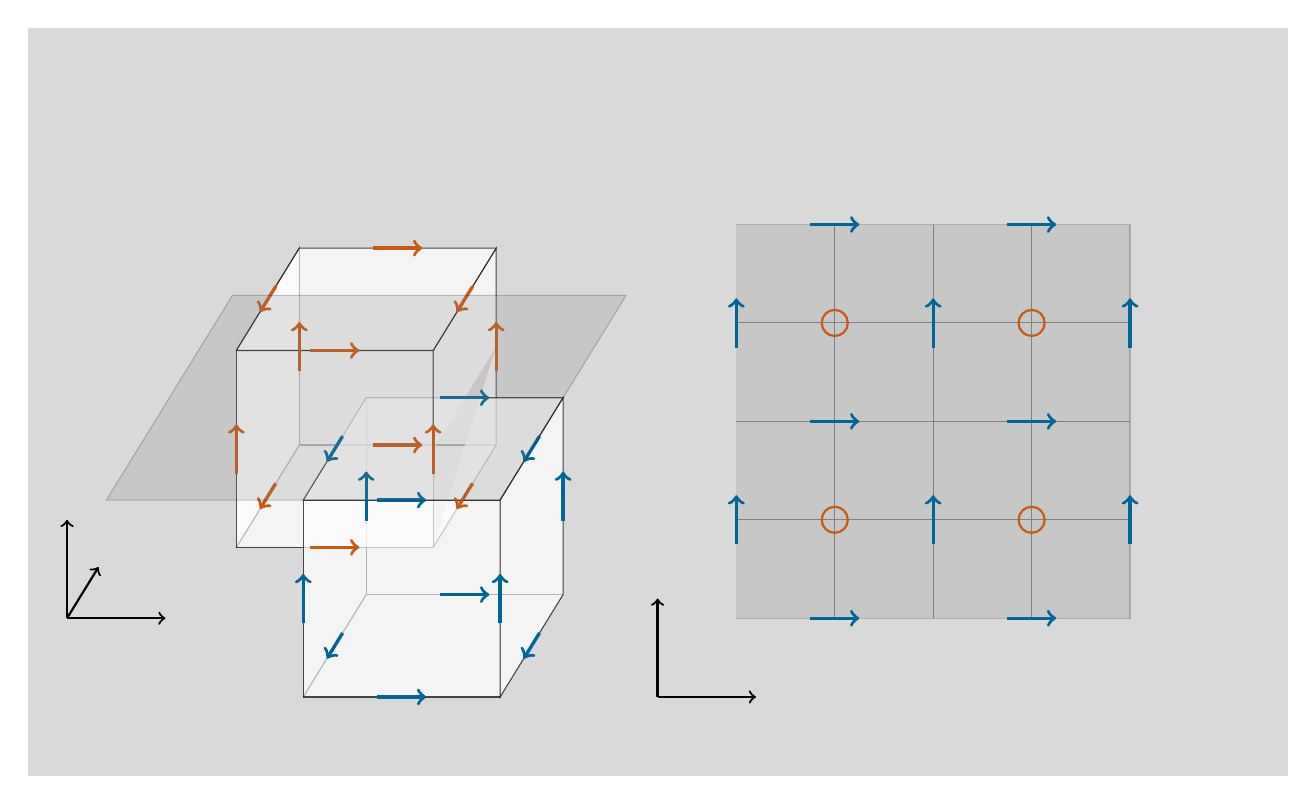
\begin{tikzpicture}[scale=0.5]
    \def\dxx{2.5};
    \def\dxy{0};
    \def\dyx{0.8};
    \def\dyy{1.3};
    \def\dzx{0};
    \def\dzy{2.5};
  \def\bgx{-7};
  \def\bgxx{25};
  \def\bgy{-7};
  \def\bgyy{12};
  \fill[opacity=0.15] (\bgx,\bgy)rectangle(\bgxx,\bgyy);
    %red invisible
    \draw (-\dxx+3*\dyx-\dzx,-\dxy+3*\dyy-\dzy)
    --++(2*\dzx,2*\dzy);
    \draw (-\dxx+3*\dyx-\dzx,-\dxy+3*\dyy-\dzy)
    --++(2*\dxx,2*\dxy);
    \draw (-\dxx+3*\dyx-\dzx,-\dxy+3*\dyy-\dzy)
    --++(-2*\dyx,-2*\dyy);
    %blue invisible
    \draw (2*\dyx,2*\dyy)
    --++(-2*\dzx,-2*\dzy);
    \draw (2*\dyx-2*\dzx,2*\dyy-2*\dzy)
    --++(-2*\dyx,-2*\dyy);
    \draw (2*\dyx-2*\dzx,2*\dyy-2*\dzy)
    --++(2*\dxx,2*\dxy);
    \draw[fill=white,opacity=0.7] (\dyx-\dzy,\dyy-\dzy)
    --++(2*\dyx,2*\dyy)%--++(-\dzx,-\dzy)
    --++(2*\dzx,2*\dzy)
    --++(-2*\dyx,-2*\dyy);
    \draw[fill=white,opacity=0.7] (2*\dxx+\dyx-\dzy,2*\dxy+\dyy-\dzy)
    --++(2*\dyx,2*\dyy)%--++(-\dzx,-\dzy)
    --++(\dzx,\dzy);
    \draw[fill=white,opacity=0.7] (-\dxx+\dyx,-\dxy+\dyy)
    --++(-\dzx,-\dzy)%--++(-\dzx,-\dzy)
    --++(2*\dxx,2*\dxy)
    --++(\dzx,\dzy);
    \draw[fill=white,opacity=0.7] (2*\dxx+\dyx,2*\dxy+\dyy)
    --++(\dyx,\dyy)
    --++(-\dxx,-\dxy)--++(-\dxx,-\dxy)
    --++(-\dyx,-\dyy);
    \draw[fill=white,opacity=0.7] (-\dxx+\dyx,-\dxy+\dyy)
    --++(\dzx,\dzy)%--++(\dzx,\dzy)
    --++(\dxx,\dxy)--++(\dxx,\dxy)
    --++(-\dzx,-\dzy);%--++(-\dzx,-\dzy)
    \draw[fill=white,opacity=0.7] (\dxx+\dyx,\dxy+\dyy)
    --++(\dzx,\dzy)%--++(-\dzx,-\dzy)
    --++(2*\dyx,2*\dyy)
    --++(-\dzx,-\dzy);
    \draw[fill=white,opacity=0.7] (2*\dxx+\dyx,2*\dxy+\dyy)
    --++(-\dyx,-\dyy)
    --++(-\dxx,-\dxy)--++(-\dxx,-\dxy)
    --++(\dyx,\dyy);
    %red top 
    \draw[fill=white,opacity=0.7] (-\dxx+\dzx+\dyx,-\dxy+\dzy+\dyy)
    --++(2*\dxx,2*\dxy)
    --++(2*\dyx,2*\dyy)
    --++(-2*\dxx,-2*\dxy)
    --++(-2*\dyx,-2*\dyy);

    %blue front, right
    \draw[fill=white,opacity=0.7] (0,0)
    --++(2*\dxx,2*\dxy)
    --++(-2*\dzx,-2*\dzy)
    --++(-2*\dxx,-2*\dxy)
    --++(2*\dzx,2*\dzy);
    \draw[fill=white,opacity=0.7] (2*\dxx,2*\dxy)
    --++(2*\dyx,2*\dyy)
    --++(-2*\dzx,-2*\dzy)
    --++(-2*\dyx,-2*\dyy)
    --++(2*\dzx,2*\dzy);
  


    \draw[emph1,->,very thick] (1.25*\dyx,1.25*\dyy)--++(-0.5*\dyx,-0.5*\dyy);
    \draw[emph1,->,very thick] (1.25*\dyx+2*\dxx,1.25*\dyy+2*\dxy)--++(-0.5*\dyx,-0.5*\dyy);
    \draw[emph1,->,very thick] (1.25*\dyx-2*\dzx,1.25*\dyy-2*\dzy)--++(-0.5*\dyx,-0.5*\dyy);
    \draw[emph1,->,very thick] (1.25*\dyx-2*\dzx+2*\dxx,1.25*\dyy-2*\dzy+2*\dxy)--++(-0.5*\dyx,-0.5*\dyy);

    \draw[emph1,->,very thick] (0.75*\dxx,0.75*\dxy)--++(0.5*\dxx,0.5*\dxy);
    \draw[emph1,->,very thick] (0.75*\dxx+2*\dyx,0.75*\dxy+2*\dyy)--++(0.5*\dxx,0.5*\dxy);
    \draw[emph1,->,very thick] (0.75*\dxx+2*\dyx-2*\dzx,0.75*\dxy+2*\dyy-2*\dzy)--++(0.5*\dxx,0.5*\dxy);
    \draw[emph1,->,very thick] (0.75*\dxx-2*\dzx,0.75*\dxy-2*\dzy)--++(0.5*\dxx,0.5*\dxy);

    \draw[emph1,->,very thick] (-1.25*\dzx,-1.25*\dzy)--++(0.5*\dzx,0.5*\dzy);
    \draw[emph1,->,very thick] (-1.25*\dzx+2*\dxx,2*\dxy-1.25*\dzy)--++(0.5*\dzx,0.5*\dzy);
    \draw[emph1,->,very thick] (-1.25*\dzx+2*\dxx+2*\dyx,2*\dxy-1.25*\dzy+2*\dyy)--++(0.5*\dzx,0.5*\dzy);
    \draw[emph1,->,very thick] (-1.25*\dzx+2*\dyx,-1.25*\dzy+2*\dyy)--++(0.5*\dzx,0.5*\dzy);
    \begin{scope}[shift={(-\dxx+\dyx+\dzx,-\dxy+\dyy+\dzy)}]
    \draw[emph2,->,very thick] (1.25*\dyx,1.25*\dyy)--++(-0.5*\dyx,-0.5*\dyy);
    \draw[emph2,->,very thick] (1.25*\dyx+2*\dxx,1.25*\dyy+2*\dxy)--++(-0.5*\dyx,-0.5*\dyy);
    \draw[emph2,->,very thick] (1.25*\dyx-2*\dzx,1.25*\dyy-2*\dzy)--++(-0.5*\dyx,-0.5*\dyy);
    \draw[emph2,->,very thick] (1.25*\dyx-2*\dzx+2*\dxx,1.25*\dyy-2*\dzy+2*\dxy)--++(-0.5*\dyx,-0.5*\dyy);

    \draw[emph2,->,very thick] (0.75*\dxx,0.75*\dxy)--++(0.5*\dxx,0.5*\dxy);
    \draw[emph2,->,very thick] (0.75*\dxx+2*\dyx,0.75*\dxy+2*\dyy)--++(0.5*\dxx,0.5*\dxy);
    \draw[emph2,->,very thick] (0.75*\dxx+2*\dyx-2*\dzx,0.75*\dxy+2*\dyy-2*\dzy)--++(0.5*\dxx,0.5*\dxy);
    \draw[emph2,->,very thick] (0.75*\dxx-2*\dzx,0.75*\dxy-2*\dzy)--++(0.5*\dxx,0.5*\dxy);

    \draw[emph2,->,very thick] (-1.25*\dzx,-1.25*\dzy)--++(0.5*\dzx,0.5*\dzy);
    \draw[emph2,->,very thick] (-1.25*\dzx+2*\dxx,2*\dxy-1.25*\dzy)--++(0.5*\dzx,0.5*\dzy);
    \draw[emph2,->,very thick] (-1.25*\dzx+2*\dxx+2*\dyx,2*\dxy-1.25*\dzy+2*\dyy)--++(0.5*\dzx,0.5*\dzy);
    \draw[emph2,->,very thick] (-1.25*\dzx+2*\dyx,-1.25*\dzy+2*\dyy)--++(0.5*\dzx,0.5*\dzy);
    \end{scope}
    
    \draw[fill=gray,opacity=0.2] (2*\dxx,2*\dxy)
    --++(4*\dyx,4*\dyy)
    --++(-4*\dxx,-4*\dxy)
    --++(-4*\dyx,-4*\dyy)
    --++(4*\dxx,4*\dxy);

    %\draw[gray, dashed] (.5,-5)--(0.5,1)--(2.5,4)--(2.5,-2)--(.5,-5);
    \draw[thick,->](-6,-3)--++(\dxx,\dxy);
    \draw[thick,->](-6,-3)--++(\dyx,\dyy);
    \draw[thick,->](-6,-3)--++(\dzx,\dzy);
    \begin{scope}[shift={(11,-3)}]
    \def\dx{2.5};
    \def\dy{2.5};
    \draw[fill=gray,opacity=0.2] (0,0)--++(4*\dx,0)--++(0,4*\dy)--++(-4*\dx,0);
    \draw[gray] (\dx,0)--++(0,4*\dy);
    \draw[gray] (2*\dx,0)--++(0,4*\dy);
    \draw[gray] (3*\dx,0)--++(0,4*\dy);
    \draw[gray] (0,\dy)--++(4*\dx,0);
    \draw[gray] (0,2*\dy)--++(4*\dx,0);
    \draw[gray] (0,3*\dy)--++(4*\dx,0);

    \draw[emph1,->,very thick] (\dx-0.25*\dx,0)--++(0.5*\dx,0);
    \draw[emph1,->,very thick] (3*\dx-0.25*\dx,0)--++(0.5*\dx,0);


    \draw[emph1,->,very thick] (\dx-0.25*\dx,2*\dy)--++(0.5*\dx,0);
    \draw[emph1,->,very thick] (3*\dx-0.25*\dx,2*\dy)--++(0.5*\dx,0);


    \draw[emph1,->,very thick] (\dx-0.25*\dx,4*\dy)--++(0.5*\dx,0);
    \draw[emph1,->,very thick] (3*\dx-0.25*\dx,4*\dy)--++(0.5*\dx,0);

    \draw[emph1,->,very thick] (0,\dy-0.25*\dy)--++(0,0.5*\dy);
    \draw[emph1,->,very thick] (0,3*\dy-0.25*\dy,0)--++(0,0.5*\dy);

    \draw[emph1,->,very thick] (2*\dx,\dy-0.25*\dy)--++(0,0.5*\dy);
    \draw[emph1,->,very thick] (2*\dx,3*\dy-0.25*\dy,0)--++(0,0.5*\dy);

    \draw[emph1,->,very thick] (4*\dx,\dy-0.25*\dy)--++(0,0.5*\dy);
    \draw[emph1,->,very thick] (4*\dx,3*\dy-0.25*\dy,0)--++(0,0.5*\dy);

    \node[circle,thick,draw=emph2] at (\dx,\dy){};
    \node[circle,thick,draw=emph2] at (3*\dx,\dy){};
    \node[circle,thick,draw=emph2] at (\dx,3*\dy){};
    \node[circle,thick,draw=emph2] at (3*\dx,3*\dy){};
    %axis
    \draw[thick,->](-2,-2)--++(\dx,0);
    \draw[thick,->](-2,-2)--++(0,\dy);
    \end{scope}
  \end{tikzpicture}
      

\tikzsetnextfilename{primal_dual_quad}
  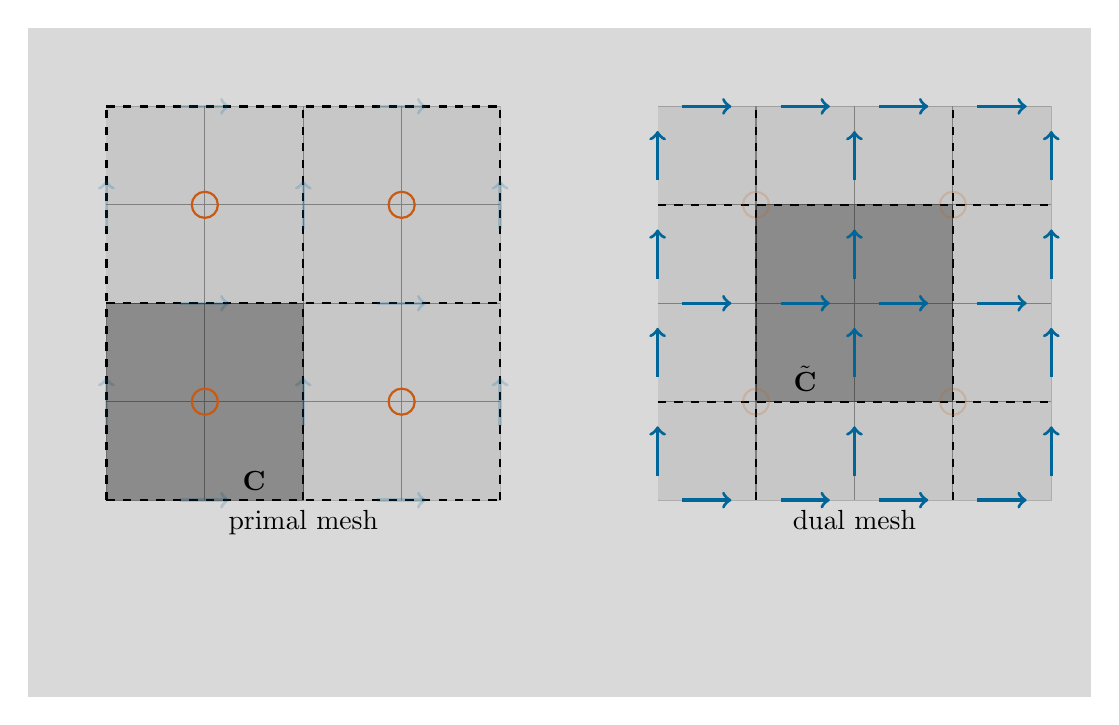
\begin{tikzpicture}[scale=0.5]
    \def\dx{2.5};
    \def\dy{2.5};
  \def\bgx{-2};
  \def\bgxx{25};
  \def\bgy{-5};
  \def\bgyy{12};
  \fill[opacity=0.15] (\bgx,\bgy)rectangle(\bgxx,\bgyy);
    \draw[fill=gray,opacity=0.2] (0,0)--++(4*\dx,0)--++(0,4*\dy)--++(-4*\dx,0);
    \draw[gray] (\dx,0)--++(0,4*\dy);
    \draw[gray] (2*\dx,0)--++(0,4*\dy);
    \draw[gray] (3*\dx,0)--++(0,4*\dy);
    \draw[gray] (0,\dy)--++(4*\dx,0);
    \draw[gray] (0,2*\dy)--++(4*\dx,0);
    \draw[gray] (0,3*\dy)--++(4*\dx,0);

    \draw[black,thick,dashed] (0,0)--++(4*\dx,0);
    \draw[black,thick,dashed] (0,0)--++(0,4*\dy);
    \draw[black,thick,dashed] (2*\dx,0)--++(0,4*\dy);
    \draw[black,thick,dashed] (4*\dx,0)--++(0,4*\dy);
    \draw[black,thick,dashed] (0,2*\dy)--++(4*\dx,0);
    \draw[black,thick,dashed] (0,4*\dy)--++(4*\dx,0);



    \draw[emph1,->,very thick,opacity=0.2] (\dx-0.25*\dx,0)--++(0.5*\dx,0);
    \draw[emph1,->,very thick,opacity=0.2] (3*\dx-0.25*\dx,0)--++(0.5*\dx,0);
    \draw[emph1,->,very thick,opacity=0.2] (\dx-0.25*\dx,2*\dy)--++(0.5*\dx,0);
    \draw[emph1,->,very thick,opacity=0.2] (3*\dx-0.25*\dx,2*\dy)--++(0.5*\dx,0);
    \draw[emph1,->,very thick,opacity=0.2] (\dx-0.25*\dx,4*\dy)--++(0.5*\dx,0);
    \draw[emph1,->,very thick,opacity=0.2] (3*\dx-0.25*\dx,4*\dy)--++(0.5*\dx,0);
    \draw[emph1,->,very thick,opacity=0.2] (0,\dy-0.25*\dy)--++(0,0.5*\dy);
    \draw[emph1,->,very thick,opacity=0.2] (0,3*\dy-0.25*\dy,0)--++(0,0.5*\dy);
    \draw[emph1,->,very thick,opacity=0.2] (2*\dx,\dy-0.25*\dy)--++(0,0.5*\dy);
    \draw[emph1,->,very thick,opacity=0.2] (2*\dx,3*\dy-0.25*\dy,0)--++(0,0.5*\dy);
    \draw[emph1,->,very thick,opacity=0.2] (4*\dx,\dy-0.25*\dy)--++(0,0.5*\dy);
    \draw[emph1,->,very thick,opacity=0.2] (4*\dx,3*\dy-0.25*\dy,0)--++(0,0.5*\dy);
    \draw[fill=black,opacity=0.3](0,0)--++(2*\dx,0)--++(0,2*\dy)--++(-2*\dx,0)--++(0,-2*\dy);
    \node[above] at (1.5*\dx,0){$\mathbf C$};
    \node[circle,thick,draw=emph2] at (\dx,\dy){};
    \node[circle,thick,draw=emph2] at (3*\dx,\dy){};
    \node[circle,thick,draw=emph2] at (\dx,3*\dy){};
    \node[circle,thick,draw=emph2] at (3*\dx,3*\dy){};
    \node[below] at (2*\dx,0){primal mesh};
    \begin{scope}[shift={(14,0)}]
    \def\dx{2.5};
    \def\dy{2.5};
    \draw[fill=gray,opacity=0.2] (0,0)--++(4*\dx,0)--++(0,4*\dy)--++(-4*\dx,0);
    \draw[gray] (\dx,0)--++(0,4*\dy);
    \draw[gray] (2*\dx,0)--++(0,4*\dy);
    \draw[gray] (3*\dx,0)--++(0,4*\dy);
    \draw[gray] (0,\dy)--++(4*\dx,0);
    \draw[gray] (0,2*\dy)--++(4*\dx,0);
    \draw[gray] (0,3*\dy)--++(4*\dx,0);

    \draw[black,thick,dashed] (1*\dx,0)--++(0,4*\dy);
    \draw[black,thick,dashed] (3*\dx,0)--++(0,4*\dy);
    \draw[black,thick,dashed] (0,1*\dy)--++(4*\dx,0);
    \draw[black,thick,dashed] (0,3*\dy)--++(4*\dx,0);
    \draw[fill=black,opacity=0.3](\dx,\dy)--++(2*\dx,0)--++(0,2*\dy)--++(-2*\dx,0)--++(0,-2*\dy);
    \node[above] at (1.5*\dx,1*\dy){$\tilde {\mathbf C}$};

    \draw[emph1,->,very thick] (0.5*\dx-0.25*\dx,0)--++(0.5*\dx,0);
    \draw[emph1,->,very thick] (1.5*\dx-0.25*\dx,0)--++(0.5*\dx,0);
    \draw[emph1,->,very thick] (2.5*\dx-0.25*\dx,0)--++(0.5*\dx,0);
    \draw[emph1,->,very thick] (3.5*\dx-0.25*\dx,0)--++(0.5*\dx,0);
    \draw[emph3,->,very thick,opacity=0] (\dx-0.25*\dx,0)--++(0.5*\dx,0);
    \draw[emph3,->,very thick,opacity=0] (3.5*\dx-0.25*\dx,4*\dy)--++(0.5*\dx,0);

    \draw[emph1,->,very thick] (0.5*\dx-0.25*\dx,2*\dy)--++(0.5*\dx,0);
    \draw[emph1,->,very thick] (1.5*\dx-0.25*\dx,2*\dy)--++(0.5*\dx,0);
    \draw[emph1,->,very thick] (2.5*\dx-0.25*\dx,2*\dy)--++(0.5*\dx,0);
    \draw[emph1,->,very thick] (3.5*\dx-0.25*\dx,2*\dy)--++(0.5*\dx,0);

    \draw[emph1,->,very thick] (0.5*\dx-0.25*\dx,4*\dy)--++(0.5*\dx,0);
    \draw[emph1,->,very thick] (1.5*\dx-0.25*\dx,4*\dy)--++(0.5*\dx,0);
    \draw[emph1,->,very thick] (2.5*\dx-0.25*\dx,4*\dy)--++(0.5*\dx,0);
    \draw[emph1,->,very thick] (3.5*\dx-0.25*\dx,4*\dy)--++(0.5*\dx,0);

    \draw[emph1,->,very thick] (0,0.5*\dy-0.25*\dy)--++(0,0.5*\dy);
    \draw[emph1,->,very thick] (0,1.5*\dy-0.25*\dy)--++(0,0.5*\dy);
    \draw[emph1,->,very thick] (0,2.5*\dy-0.25*\dy)--++(0,0.5*\dy);
    \draw[emph1,->,very thick] (0,3.5*\dy-0.25*\dy,0)--++(0,0.5*\dy);

    \draw[emph1,->,very thick] (2*\dx,0.5*\dy-0.25*\dy)--++(0,0.5*\dy);
    \draw[emph1,->,very thick] (2*\dx,1.5*\dy-0.25*\dy)--++(0,0.5*\dy);
    \draw[emph1,->,very thick] (2*\dx,2.5*\dy-0.25*\dy)--++(0,0.5*\dy);
    \draw[emph1,->,very thick] (2*\dx,3.5*\dy-0.25*\dy,0)--++(0,0.5*\dy);

    \draw[emph1,->,very thick] (4*\dx,0.5*\dy-0.25*\dy)--++(0,0.5*\dy);
    \draw[emph1,->,very thick] (4*\dx,1.5*\dy-0.25*\dy)--++(0,0.5*\dy);
    \draw[emph1,->,very thick] (4*\dx,2.5*\dy-0.25*\dy)--++(0,0.5*\dy);
    \draw[emph1,->,very thick] (4*\dx,3.5*\dy-0.25*\dy,0)--++(0,0.5*\dy);

    \node[circle,thick,draw=emph2,opacity=0.2] at (\dx,\dy){};
    \node[circle,thick,draw=emph2,opacity=0.2] at (3*\dx,\dy){};
    \node[circle,thick,draw=emph2,opacity=0.2] at (\dx,3*\dy){};
    \node[circle,thick,draw=emph2,opacity=0.2] at (3*\dx,3*\dy){};
    %axis
    %\draw[thick,->](-2,-2)--++(\dx,0);
    %\draw[thick,->](-2,-2)--++(0,\dy);
    \node[below] at (2*\dx,0){dual mesh};
    \end{scope}
  \end{tikzpicture}%


\tikzsetnextfilename{dual_mesh_left}
        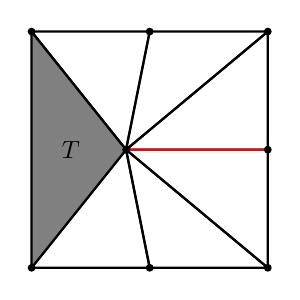
\begin{tikzpicture}[thick,scale=3.0, every node/.style={scale=3.0}]
        \coordinate (p1) at (0.0,0.0);
        \coordinate (p2) at (0.5,0.0);
        \coordinate (p3) at (1.0,0.0);
        \coordinate (p4) at (0.4,0.5);
        \coordinate (p5) at (1.0,0.5);
        \coordinate (p6) at (0.0,1.0);
        \coordinate (p7) at (0.5,1.0);
        \coordinate (p8) at (1.0,1.0);  
        \draw (p1) -- (p2) -- (p4) -- (p1);
        \draw[fill=gray] (p1) -- (p4) -- (p6) -- (p1);
        \draw (p4) -- (p6) -- (p7) -- (p4);
        \draw (p4) -- (p2) -- (p3) -- (p4);
        \draw (p4) -- (p3) -- (p5) -- (p4);
        \draw (p4) -- (p7) -- (p8) -- (p4);
        \draw (p4) -- (p8) -- (p5) -- (p4);
        \draw[color=red] (p4) -- (p5);
        % \node[scale=0.3] at (0.4+0.07,1/2+0.1) {$\mathbf{v}$};
        % \node[scale=0.3,color=red,thick] at (3/4,1/2+0.05) {$E$};
        \node[scale=0.3] at (1/6,1/2) {$T$};
        \node[circle,fill,scale=0.1] at (p1) {};
        \node[circle,fill,scale=0.1] at (p2) {};
        \node[circle,fill,scale=0.1] at (p3) {};
        \node[circle,fill,scale=0.1] at (p4) {};
        \node[circle,fill,scale=0.1] at (p5) {};
        \node[circle,fill,scale=0.1] at (p6) {};
        \node[circle,fill,scale=0.1] at (p7) {};
        \node[circle,fill,scale=0.1] at (p8) {};  
        \end{tikzpicture}
\tikzsetnextfilename{dual_mesh_center}

        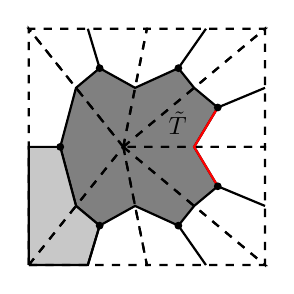
\begin{tikzpicture}[thick,scale=3.0, every node/.style={scale=3.0}]

          \coordinate (p1) at (0.0,0.0);
          \coordinate (p2) at (0.5,0.0);
          \coordinate (p3) at (1.0,0.0);
          \coordinate (p4) at (0.4,0.5);
          \coordinate (p5) at (1.0,0.5);
          \coordinate (p6) at (0.0,1.0);
          \coordinate (p7) at (0.5,1.0);
          \coordinate (p8) at (1.0,1.0);   
          \coordinate (p9) at (0.3000,0.1667);
          \coordinate (p10) at (0.1333,0.5000);
          \coordinate (p11) at (0.3000,0.8333);
          \coordinate (p12) at (0.6333,0.1667);
          \coordinate (p13) at (0.8000,0.3333);
          \coordinate (p14) at (0.8000,0.6667);
          \coordinate (p15) at (0.6333,0.8333);
          \coordinate (p16) at (0.2500,0);
          \coordinate (p17) at (0.2000,0.2500);
          \coordinate (p18) at (0.0,0.5000);
          \coordinate (p19) at (0.7500,0);
          \coordinate (p20) at (0.4500,0.2500);
          \coordinate (p21) at (0.7000,0.2500);
          \coordinate (p22) at (1.0000,0.2500);
          \coordinate (p23) at (0.7000,0.5000);
          \coordinate (p24) at (0.2000,0.7500);
          \coordinate (p25) at (0.4500,0.7500);
          \coordinate (p26) at (0.7000,0.7500);
          \coordinate (p27) at (1.0000,0.7500);
          \coordinate (p28) at (0.2500,1.0000);
          \coordinate (p29) at (0.7500,1.0000);
          \draw[fill=gray] (p13) -- (p23) -- (p14) -- (p26) -- (p15) -- (p25) -- (p11) -- (p24) --
                           (p10) -- (p17) -- (p9) -- (p20) -- (p12) -- (p21) -- (p13);
          \draw[fill=lightgray] (p1) -- (p16) -- (p9) -- (p17) -- (p10) -- (p18) -- (p1);
          \draw[dashed] (p1) -- (p2) -- (p4) -- (p1);
          \draw[dashed] (p1) -- (p4) -- (p6) -- (p1);
          \draw[dashed] (p4) -- (p6) -- (p7) -- (p4);
          \draw[dashed] (p4) -- (p2) -- (p3) -- (p4);
          \draw[dashed] (p4) -- (p3) -- (p5) -- (p4);
          \draw[dashed] (p4) -- (p7) -- (p8) -- (p4);
          \draw[dashed] (p4) -- (p8) -- (p5) -- (p4);
        \draw[color=black] (p16) -- (p9);
        \draw[color=black] (p19) -- (p12);
        \draw[color=black] (p22) -- (p13);
        \draw[color=black] (p27) -- (p14);
        \draw[color=black] (p29) -- (p15);
        \draw[color=black] (p28) -- (p11);
        \draw[color=black] (p18) -- (p10);
        \draw[color=red] (p13) -- (p23) -- (p14);
        \node[circle,fill,scale=0.1] at (p9) {};
        \node[circle,fill,scale=0.1] at (p10) {};
        \node[circle,fill,scale=0.1] at (p11) {};
        \node[circle,fill,scale=0.1] at (p12) {};
        \node[circle,fill,scale=0.1] at (p13) {};
        \node[circle,fill,scale=0.1] at (p14) {};
        \node[circle,fill,scale=0.1] at (p15) {}; 
        \node[scale=0.3] at (1/2+0.13,1/2+0.1) {$\tilde{T}$};
        % \node[scale=0.3,thick,color=red] at (5/6,1/2+0.07) {$\tilde{E}$};
        % \node[scale=0.3] at (1/9,3/7) {$\tilde{\mathbf{v}}$};
        \end{tikzpicture}
\tikzsetnextfilename{dual_mesh_right}
        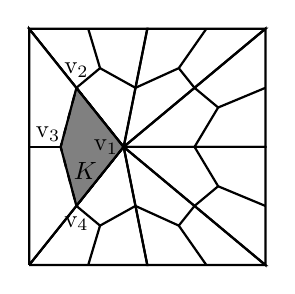
\begin{tikzpicture}[thick,scale=3.0, every node/.style={scale=3.0}]
          \coordinate (p1) at (0.0,0.0);
          \coordinate (p2) at (0.5,0.0);
          \coordinate (p3) at (1.0,0.0);
          \coordinate (p4) at (0.4,0.5);
          \coordinate (p5) at (1.0,0.5);
          \coordinate (p6) at (0.0,1.0);
          \coordinate (p7) at (0.5,1.0);
          \coordinate (p8) at (1.0,1.0);   
          \coordinate (p9) at (0.3000,0.1667);
          \coordinate (p10) at (0.1333,0.5000);
          \coordinate (p11) at (0.3000,0.8333);
          \coordinate (p12) at (0.6333,0.1667);
          \coordinate (p13) at (0.8000,0.3333);
          \coordinate (p14) at (0.8000,0.6667);
          \coordinate (p15) at (0.6333,0.8333);
          \coordinate (p16) at (0.2500,0);
          \coordinate (p17) at (0.2000,0.2500);
          \coordinate (p18) at (0,0.5000);
          \coordinate (p19) at (0.7500,0);
          \coordinate (p20) at (0.4500,0.2500);
          \coordinate (p21) at (0.7000,0.2500);
          \coordinate (p22) at (1.0000,0.2500);
          \coordinate (p23) at (0.7000,0.5000);
          \coordinate (p24) at (0.2000,0.7500);
          \coordinate (p25) at (0.4500,0.7500);
          \coordinate (p26) at (0.7000,0.7500);
          \coordinate (p27) at (1.0000,0.7500);
          \coordinate (p28) at (0.2500,1.0000);
          \coordinate (p29) at (0.7500,1.0000);
          \draw[dashed,fill=gray] (p4) -- (p24) -- (p10) --
                                  (p17) -- (p4);
          \draw            (p13) -- (p23) -- (p14) -- (p26) -- (p15) -- 
                           (p25) -- (p11) -- (p24) -- (p10) -- (p17) -- 
                           (p9) -- (p20) -- (p12) -- (p21) -- (p13);
          \draw (p1) -- (p2) -- (p4) -- (p1);
          \draw (p1) -- (p4) -- (p6) -- (p1);
          \draw (p4) -- (p6) -- (p7) -- (p4);
          \draw (p4) -- (p2) -- (p3) -- (p4);
          \draw (p4) -- (p3) -- (p5) -- (p4);
          \draw (p4) -- (p7) -- (p8) -- (p4);
          \draw (p4) -- (p8) -- (p5) -- (p4);
        \draw[color=black] (p16) -- (p9);
        \draw[color=black] (p19) -- (p12);
        \draw[color=black] (p22) -- (p13);
        \draw[color=black] (p27) -- (p14);
        \draw[color=black] (p29) -- (p15);
        \draw[color=black] (p28) -- (p11);
        \draw[color=black] (p18) -- (p10);
        \node[scale=0.3,left of=p4, node distance=2.5mm] (v1)  {$\mathrm v_1$};
        \node[scale=0.3,above of=p24, node distance=2.5mm] (v2) {$\mathrm v_2$};
        \node[scale=0.3,above left of=p10, node distance=2.5mm] (v3) {$\mathrm v_3$};
        \node[scale=0.3,below of=p17, node distance=2.5mm] (v4) {$\mathrm v_4$};
        % \draw[color=red] (p24) -- (p10) -- (p17);
        % \draw[color=green] (p24) -- (p4) -- (p17);
        \node[scale=0.3,below] at (0.95*1/4,0.95*1/2) {$K$};
        % \node[scale=0.3,thick,color=red] at (1/8,1/3) {$\tilde{e}$};
        % \node[scale=0.3,thick,color=green] at (1/3,2/3) {${e}$};
        \end{tikzpicture}

\end{document}:
